% !TeX spellcheck = de_DE
% !TeX TS-program = pdflatex
\documentclass{beamer}
\usepackage[utf8]{inputenc}
\usepackage[ngerman]{babel}
\usetheme{JuanLesPins}  %% Themenwahl
\usepackage{bytefield}

\usepackage{pgfpages}
\setbeamertemplate{note page}[plain]
\setbeameroption{show notes on second screen=right}

\title{RIOTOIR}
\author{Hauke, Marcel, Martin}
\date{\today}

\begin{document}
\beamertemplatenavigationsymbolsempty
\unitlength 5mm

\maketitle

\begin{frame} %%Eine Folie
  \frametitle{ RIOTOIR } %%Folientitel
  \begin{block}{\textbf{RIOT} - \textbf{O} - \textbf{IR}}
  	\begin{tabbing}
    	RIOT \= $\rightarrow$ \= RIOT\\
    	\break
    	O  	 \> $\rightarrow$ \> On\\
			\break    	
    	IR   \> $\rightarrow$ \> Infrared\\
		\end{tabbing} 
  \end{block}
\end{frame}

\begin{frame} %%Eine Folie
  \frametitle{ Überblick } %%Folientitel
  \begin{figure}
  	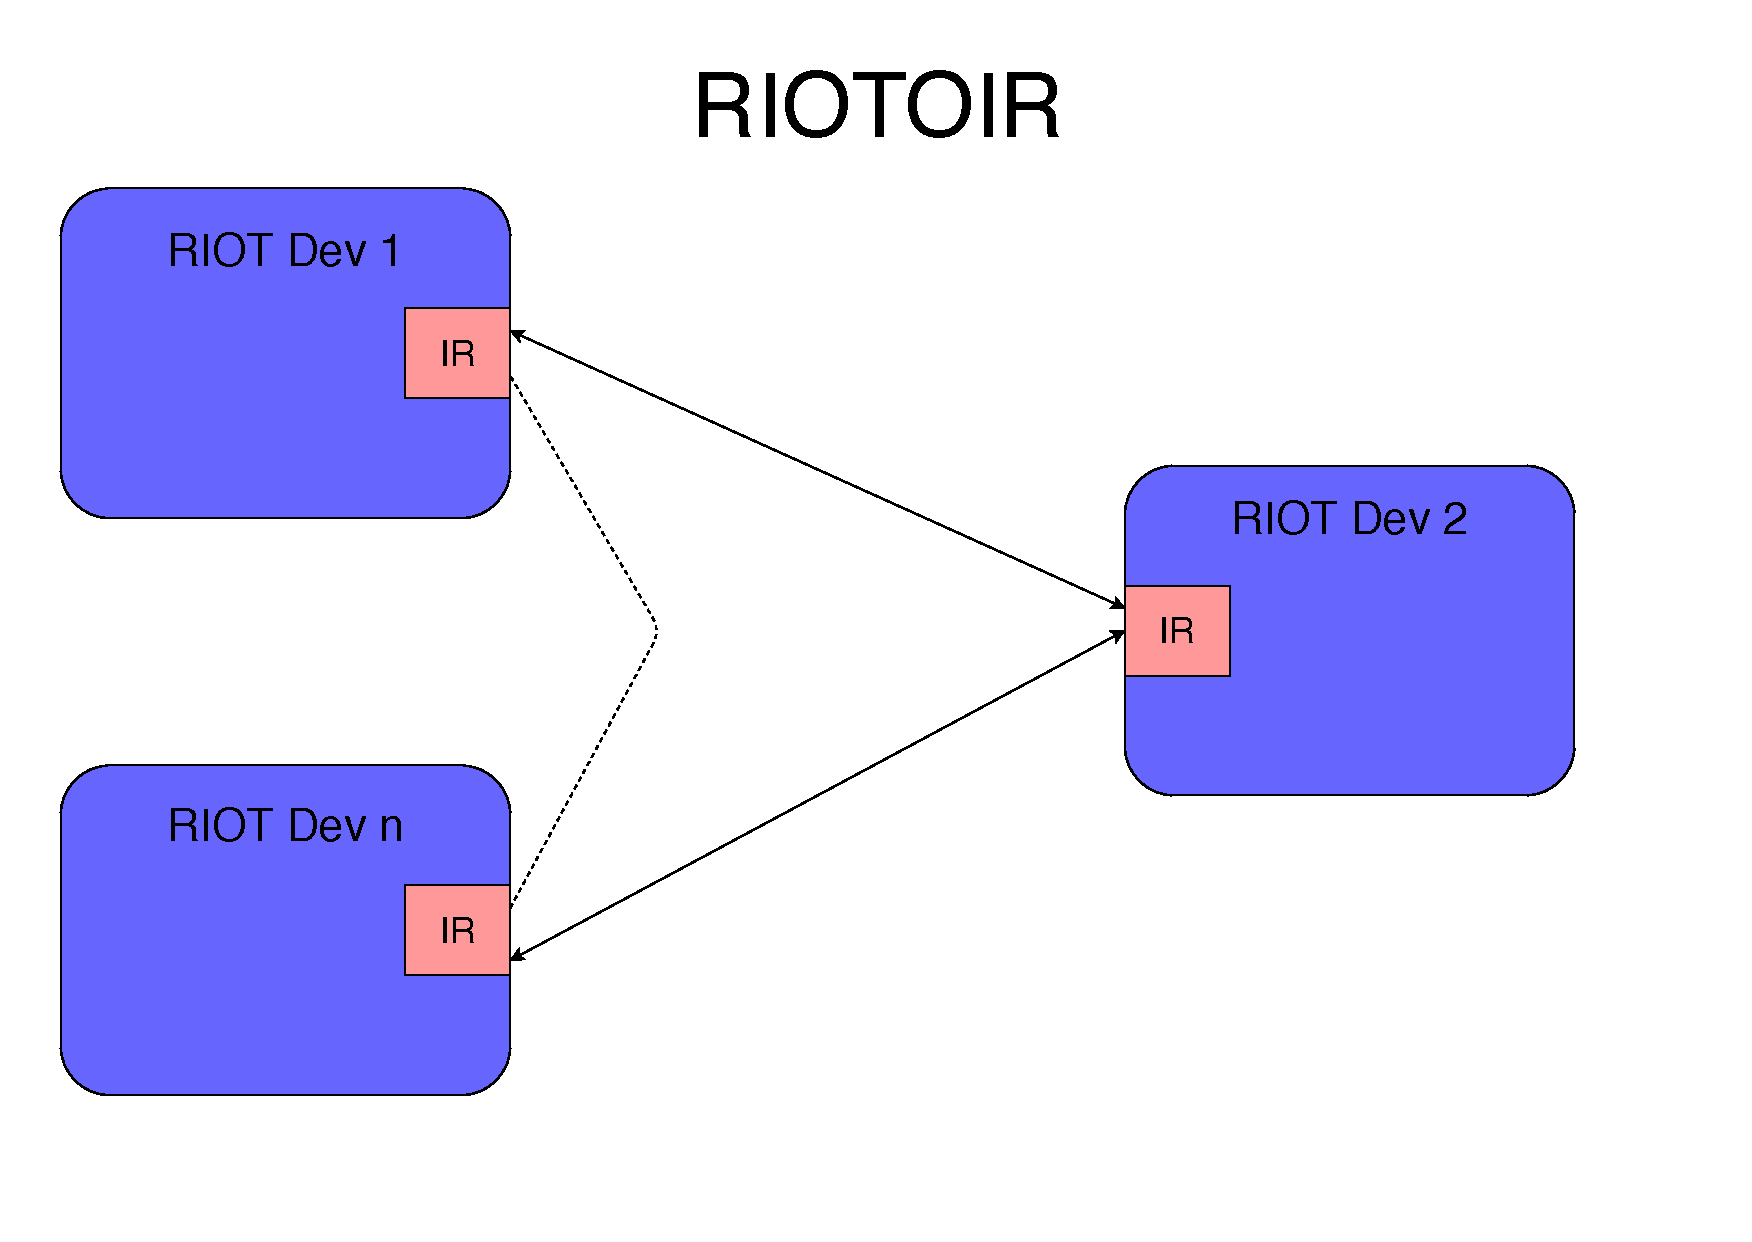
\includegraphics[scale=0.35]{Medien/RIOTOIR-Overview.pdf}
  \end{figure}
\end{frame}


\begin{frame} %%Eine Folie
  \frametitle{ Warum Infrarot } %%Folientitel
  \begin{block}{Gründe für IR-Kommunikation}
  	- Funk(WLAN, WPAN, ...) nicht möglich (z.B. Interferenzen)\\
  	\break
  	- Funk nicht gestattet, gewünscht. (z.B. Elektrosmog)\\
  	\break
  	- Keine leitungsgebundene Infrastruktur vorhanden(LAN-Kabel, ...)\\ 	
  \end{block}
\end{frame}


\begin{frame} %%Eine Folie
  \frametitle{ Use-Case } %%Folientitel
  \begin{block}{ Smart-Energy-Control }
  	\begin{columns}
			\begin{column}{6cm}
				\break
  			Der Solar-Energiezähler wird ausgelesen.\\
  			\break
  			Online werden aktuelle Wetterdaten und Prognosen geladen.\\
  		\end{column}
  		\begin{column}{3.5cm}
  			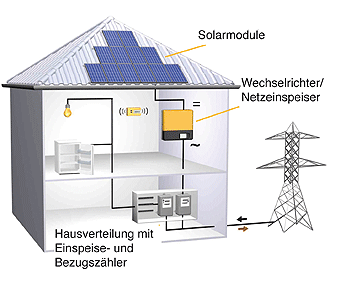
\includegraphics[scale=0.4]{Medien/solarHaus.png}\\ 
  		\end{column}
		\end{columns}
		\ \\
		\break
  	Wenn die Prognose genügend Sonnenenergie vorgibt und der aktuelle Verbrauch es zulässt, werden größere Verbraucher gestartet (WaMa, GSP, ...) 
		
  \end{block}
  
\end{frame}


\begin{frame} %%Eine Folie
  \frametitle{ Protokoll } %%Folientitel
  \begin{block}{Header}
  	\vspace{0.5cm}
  	\begin{center}
  	\begin{bytefield}{24}
			\bitheader{0-23}\\
			\bitbox{8}{Präambel} 
			\bitbox{8}{Version}			
			\bitbox{8}{Empfänger}\\
			
			\bitbox{8}{Sender}		
			\bitbox{8}{Länge}
			\bitbox{8}{Checksumme}\\
			\wordbox[tlr]{1}{Nachricht}\\
			\skippedwords\\
			\wordbox[blr]{1}{}
		\end{bytefield}
		\end{center}
		\vspace{0.3cm}
  \end{block}
\end{frame}

\note{ k }

\begin{frame} %%Eine Folie
  \frametitle{ Modulation } %%Folientitel
  \begin{figure}
  	\begin{center}
  		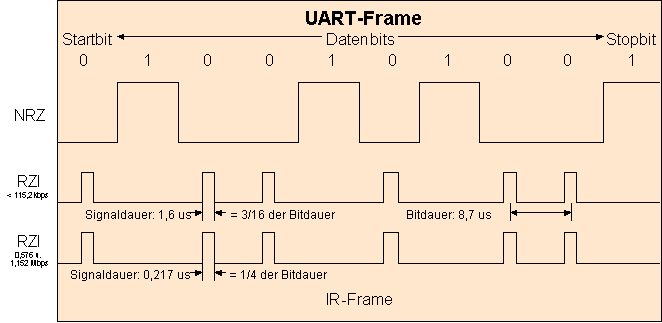
\includegraphics[scale=0.5]{Medien/Modulation.PNG}\\
  		Orientiert am Infrared Data Association $IrDA^{\textregistered}$
  	\end{center}
  \end{figure}
\end{frame}

\begin{frame}
	\frametitle{ Timing }
		\small
		\begin{tabular}{|c|c|c|c|c|}
		\hline 
		Datum  & Ereignis & Hauke & Marcel & Martin \\ 
		\hline 
		23.10. & Ready for MS2 & CRC, Zähler auslesen & Empfangen & Senden \\ 
		\hline 
		29.10. & MS 2 & & &\\
		\hline 
		27.11. & Ready for MS3 & \multicolumn{3}{|c|}{ Itegration Sender/Empfänger } \\
		&  & \multicolumn{3}{|c|}{ Integration in RIOT Netzwerkstack }\\
		&  & \multicolumn{3}{|c|}{ Testumgebung schaffen }\\
		\hline 
		03.12. & MS 3 & & & \\ 
		\hline 
	  08.01. & Project finish & \multicolumn{3}{|c|}{ Integration der Wettervorhersage } \\  
		&  & \multicolumn{3}{|c|}{ Solar-Last-Logik fertig }\\
		&  & \multicolumn{3}{|c|}{ Demo fertig }\\
		\hline
		14.01. & MS 4 & & & \\ 
		\hline 
		\end{tabular} 
\end{frame}



\end{document}